\documentclass[10pt,letterpaper]{article}
\usepackage[top=0.85in,left=0.85in,footskip=0.75in,marginparwidth=2in]{geometry}

% use Unicode characters - try changing the option if you run into troubles with special characters (e.g. umlauts)
\usepackage[utf8]{inputenc}

% tables
\usepackage{booktabs}
\usepackage{multirow}

% clean citations
\usepackage{cite}

% hyperref makes references clicky. use \url{www.example.com} or \href{www.example.com}{description} to add a clicky url
\usepackage{nameref,hyperref}

% line numbers
\usepackage[right]{lineno}

% improves typesetting in LaTeX
\usepackage{microtype}
\DisableLigatures[f]{encoding = *, family = * }

% text layout - change as needed
\raggedright
\setlength{\parindent}{0.5cm}
\textwidth 5.25in
\textheight 8.75in

% Remove % for double line spacing
%\usepackage{setspace}
%\doublespacing

% use adjustwidth environment to exceed text width (see examples in text)
\usepackage{changepage}

% adjust caption style
\usepackage[aboveskip=1pt,labelfont=bf,labelsep=period,singlelinecheck=off]{caption}

% remove brackets from references
\makeatletter
\renewcommand{\@biblabel}[1]{\quad#1.}
\makeatother

% headrule, footrule and page numbers
\usepackage{lastpage,fancyhdr,graphicx}
\usepackage{epstopdf}
\pagestyle{myheadings}
\pagestyle{fancy}
\fancyhf{}
\rfoot{\thepage/\pageref{LastPage}}
\renewcommand{\footrule}{\hrule height 2pt \vspace{2mm}}
\fancyheadoffset[L]{2.25in}
\fancyfootoffset[L]{2.25in}

% use \textcolor{color}{text} for colored text (e.g. highlight to-do areas)
\usepackage{color}

% define custom colors (this one is for figure captions)
\definecolor{Gray}{gray}{.25}

% this is required to include graphics
\usepackage{graphicx}

% use if you want to put caption to the side of the figure - see example in text
\usepackage{sidecap}

% use for have text wrap around figures
\usepackage{wrapfig}
\usepackage[pscoord]{eso-pic}
\usepackage[fulladjust]{marginnote}
\reversemarginpar

% document begins here
\begin{document}
\vspace*{0.35in}

% title goes here:
\begin{flushleft}
{\Large
\textbf\newline{CS 2881 Mini Project: Follow My Instruction and Spill the Beans Reimplementation}
}
\newline
% authors go here:
\\
Amir Amangeldi,
Zaina Edelson,
Prakrit Baruah

\end{flushleft}

\section*{Abstract}
By reimplementing the Spill the Beans paper (Qi et al.), we show that a simple instruction prompt can make instruction-tuned LMs verbatim copy retrieved text. While we could not recreate the exact findings from the paper, our results display significant data extraction from the models. Our variations on the original experiment include modifications to the system prompt, as well as efficiency tweaks to the chunking implementation.

% now start line numbers
\linenumbers

% the * after section prevents numbering
\section*{Introduction}
The Spill the Beans implementation included {x} core features:
\begin{enumerate}
    \item System Prompt:
    \item Chunking:
    \item foo:
    \item bar:
\end{enumerate}


The Spill the Beans paper showcased strong extraction scores across model size, where extraction score increased as model size increased.
\begin{figure}[ht]
\centering
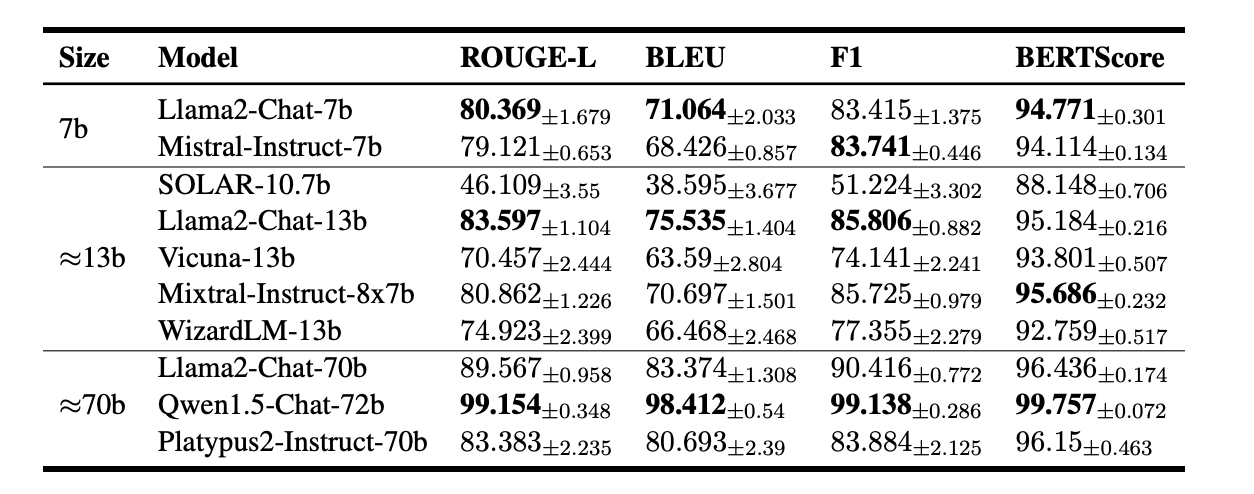
\includegraphics[width=125mm]{paper_results.png}
\caption{Published results from Spill the Beans paper} % add dummy caption - otherwise \label won't work and figure numbering will not count up
\end{figure}
% updated to PNG

%This is where your bibliography is generated. Make sure that your .bib file is actually called library.bib
\bibliography{library}

%This defines the bibliographies style. Search online for a list of available styles.
\bibliographystyle{abbrv}

\end{document}
